\chapter{Advertisement video understanding through the lens of temporal context}

In this chapter, we will explore the role of temporal context in macro-level content understanding of dynamic sources, i.e., videos. Specifically, we consider advertisement videos due to their unique narrative structures of multiple short-term temporal context changes that are linked by a longer narrative thread. In order to study the context-driven approaches, we introduce a new ads-specific benchmark called \textbf{MM-AU} with salient narrative-driven tasks for macro-level understanding i.e., topic categorization, tone transition, and social relevance. 

\section{Video Understanding}

Video Understanding aims to identify semantic elements from videos, including: \textit{environment}, \textit{objects}, \textit{actions}, \textit{events}, \textit{attributes}, \textit{concepts/themes} \cite{diba_large_2020}. Recognition of the semantic elements requires processing temporal context across different time scales, including short-term and long-term. As shown in Fig \ref{short term and long term context}, the short-term context in videos centers around visible human actions for a limited duration. However, long-term context consists of an integrated narrative spanning across multiple short-term context changes. In the case of movies, the long-term context can even span the entire duration of the movie. In this work, we primarily look at advertisement videos due to their unique narrative structure consisting of multiple short-term context changes along with long-term linkage within a limited time frame.

\begin{figure}[h!]
\centering
\subfloat[]{%
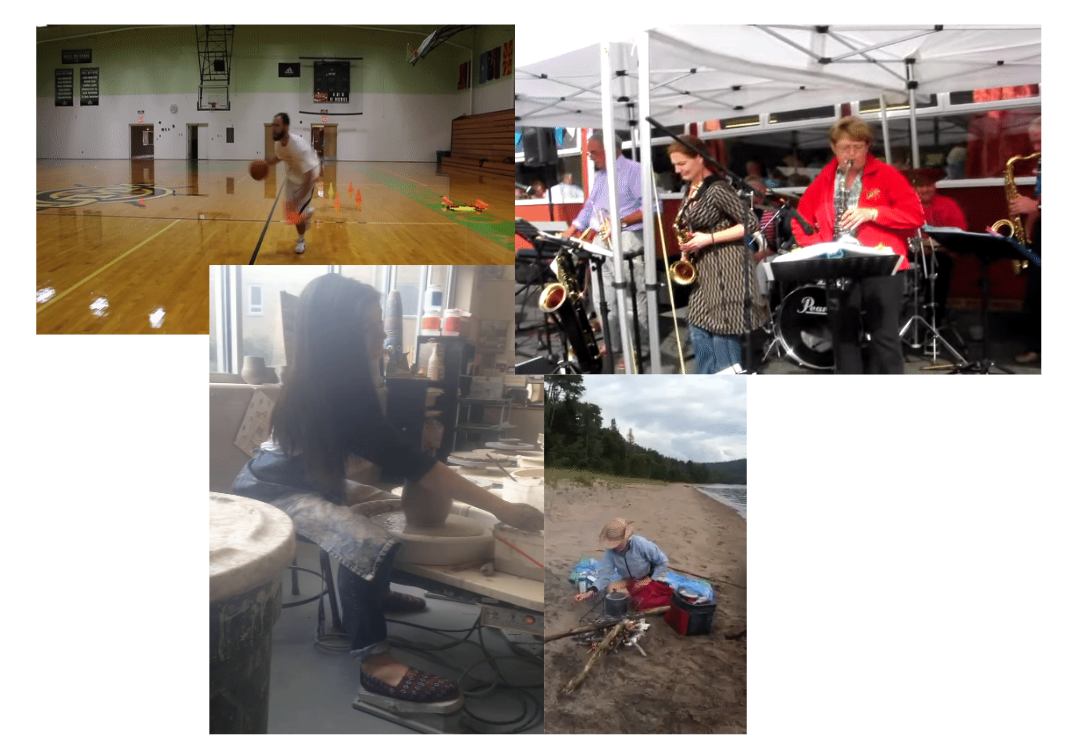
\includegraphics[width=0.5\textwidth]{figures/short_context_pictures.png}% 
\label{short context}
}
\subfloat[]{%
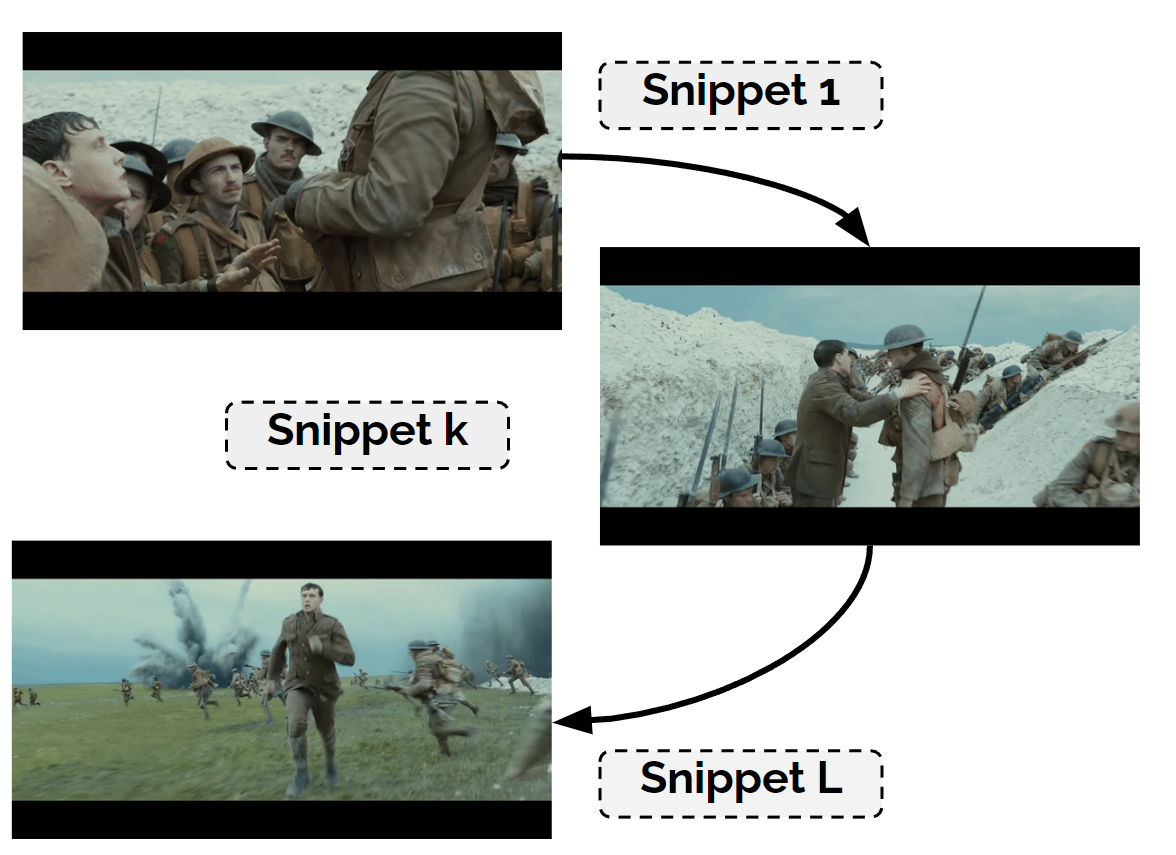
\includegraphics[width=0.5\textwidth]{figures/long_context_picture.png}%
\label{long context}
}
\caption{(a) Short-term context centered on human actions (b) Long-term context in movies useful for narrative understanding}
\label{short term and long term context}
\end{figure}

\section{Advertisements - Context transitions}

In terms of context transitions, advertisements lie between action-oriented short videos and feature-length movies. In Fig \ref{ads_structure_set}, we can see that multiple short-term context changes are happening due to the following sequence of activities/interactions:
\begin{itemize}
\item Police activity starting
\item Police chief gathering 
\item Police vehicles are getting destroyed
\item Children playing with toys 
\end{itemize}
From the sequence of events, it can be inferred that even though the short-term temporal information indicates negative situations, the overall theme revolves around toys for kids.
Thus, the temporal context information needs to be processed both locally and globally for a holistic understanding of ads at macro-level. 

\begin{figure}[h!]
\centering
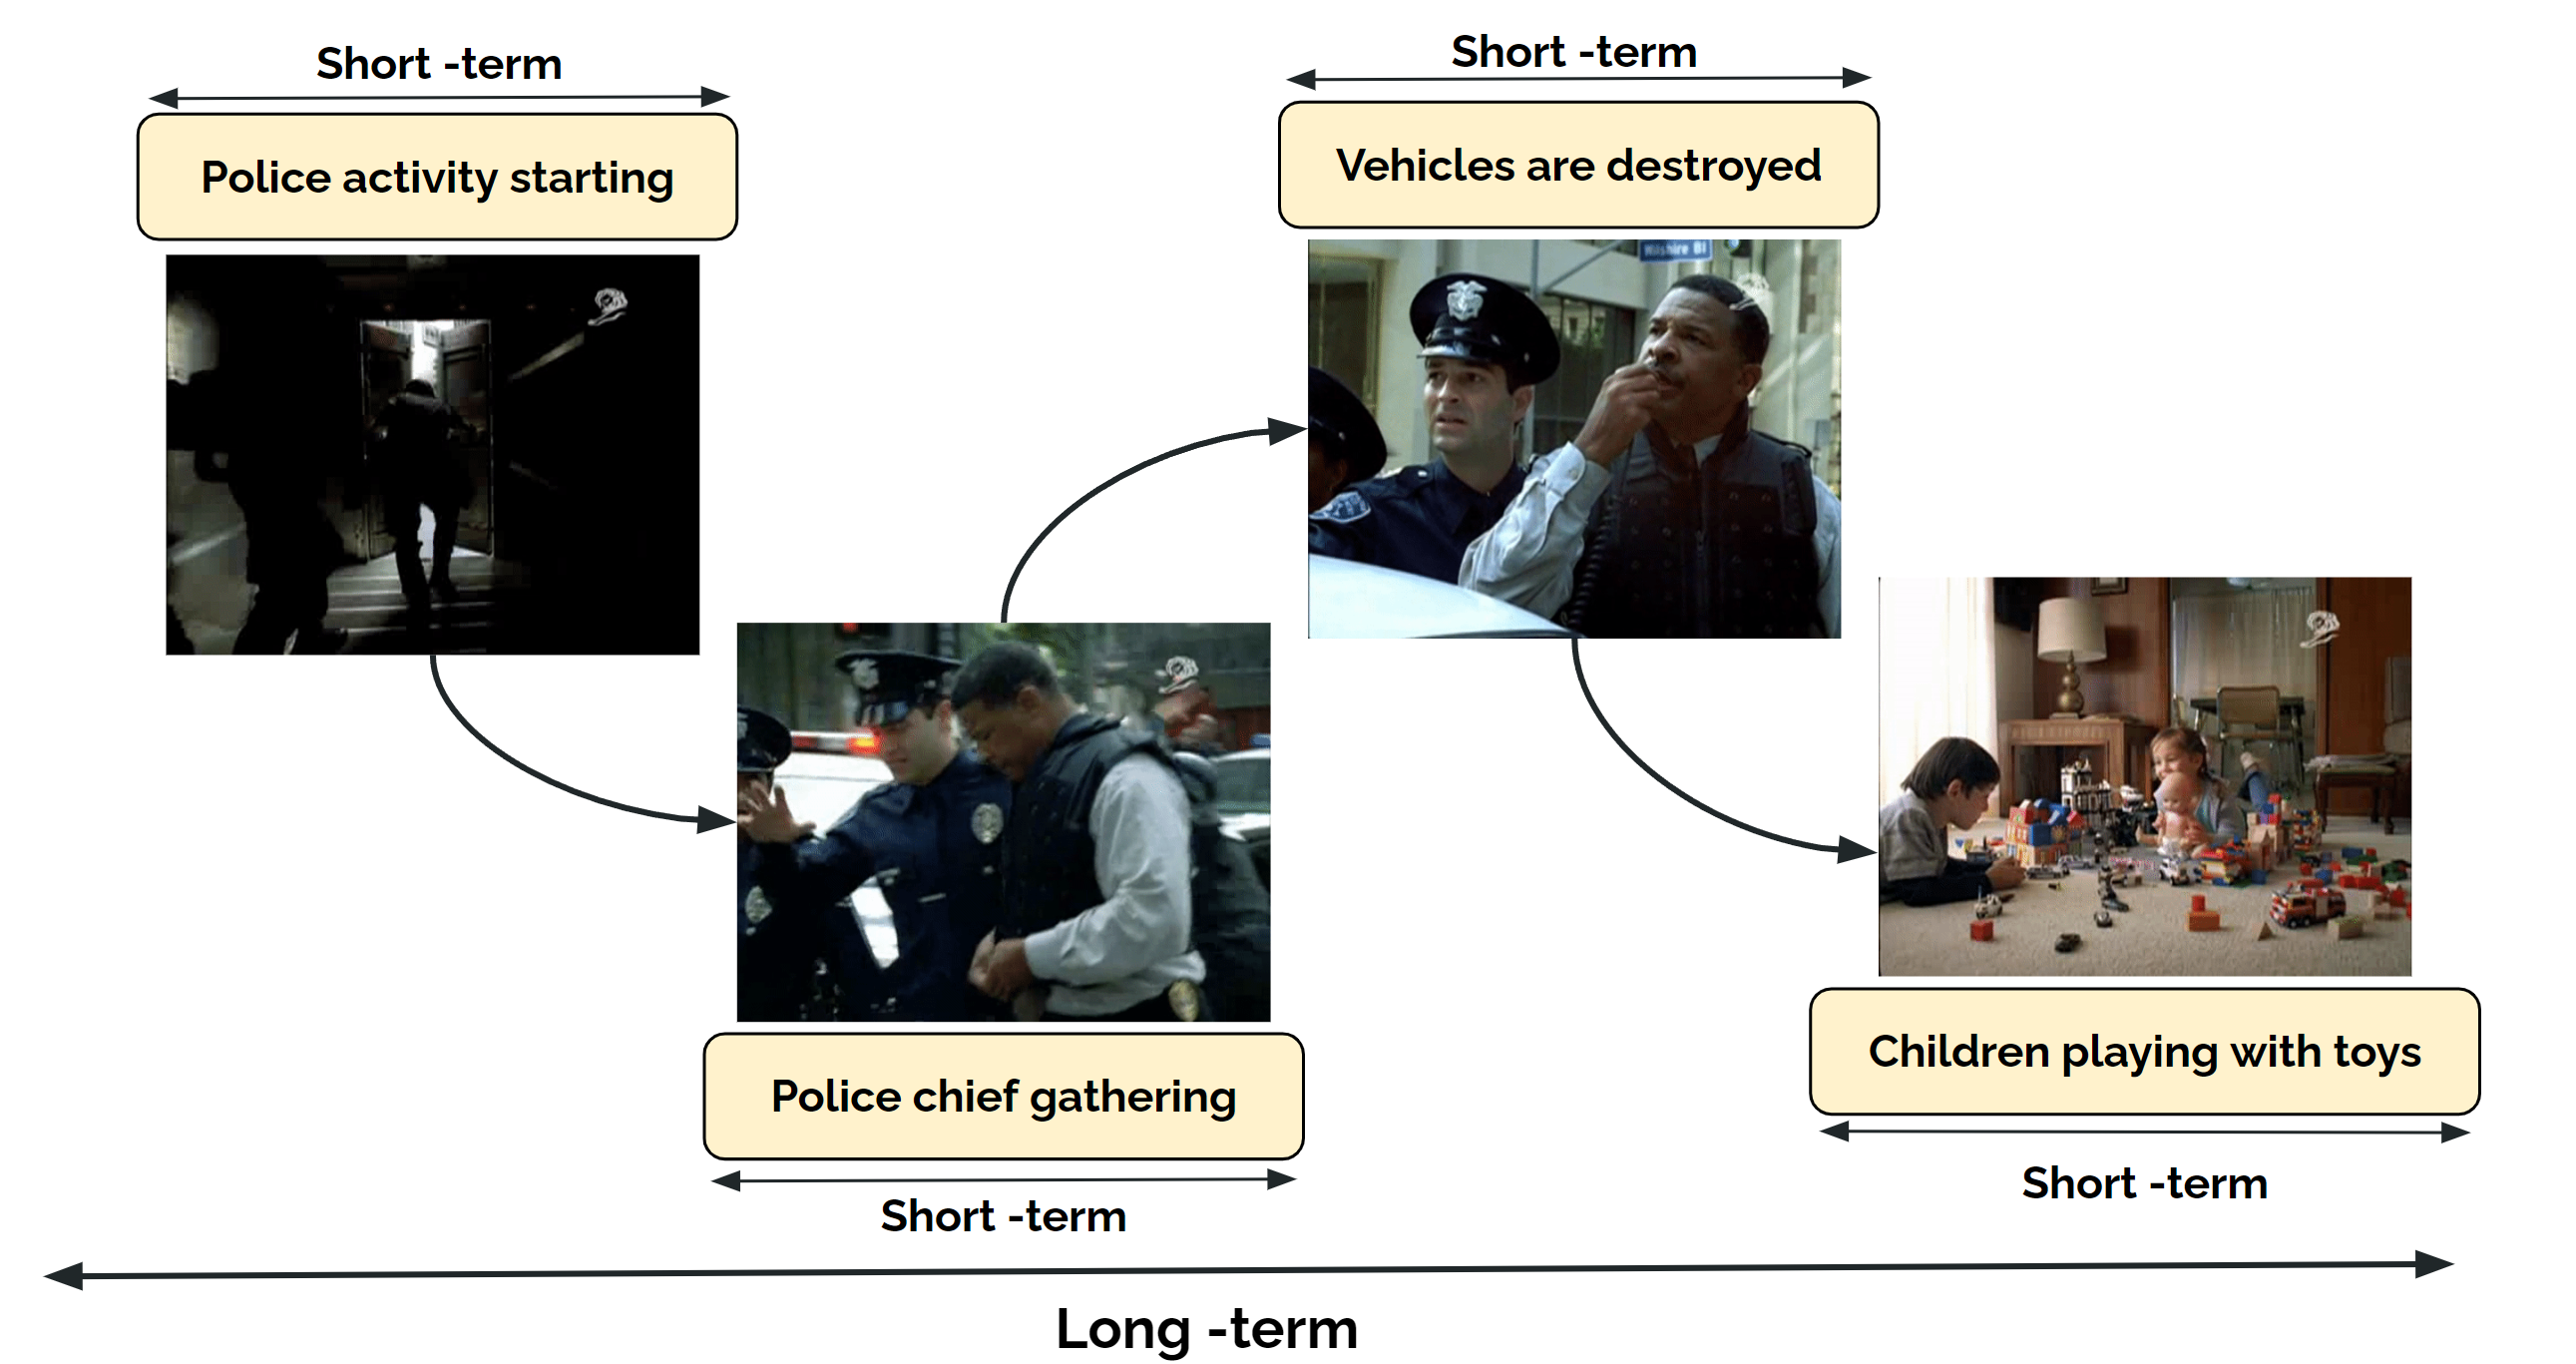
\includegraphics[width=\textwidth]{figures/ads_structure_figure.png}
\caption{Structure of advertisement video with multiple short-term context changes and overall long-term linkage}
\label{ads_structure_set}
\end{figure}



\subsection{Contextual signals as multi-modal streams:}
    \subsubsection{Visual scene context}
    \subsubsection{Auditory context}
    Background music + audio events + speech (vocalizations)
    \subsubsection{Language based context}
\section{Advertisements as medium}
\subsection{Challenges}
Mention three cases:
\begin{itemize}
\item Visual context changes sharply across shots but is tied together by an overall narrative (a diagram especially)
\item The visual narrative doesn’t happen in isolation and is usually accompanied by a transition in musical tone (the contextual signal present in the background score/music sets the mood for the advertisement)
\item The verbal cues provide descriptions of the foreground activities, including character interactions and narrations about the overall theme/topic (Language driven foreground context representations)
\section{MM-AU dataset}
\subsection{Data sources}
\subsection{Human expert-driven annotations}
\subsection{Dataset statistics}
\section{Multimodal representative tasks}
\subsection{Topic categorization}
\subsection{Tone transition}
\subsection{Absence/Presence of socially relevant cues}
\section{Progressive multimodal fusion of contextual streams}
\section{Experiments and Results}
\subsection{Language-only reasoning}
\subsection{Unimodal vs Multimodal baselines}
\section{Limitations}
\section{Conclusions}
\end{itemize}




